\documentclass[a4paper,12pt]{article}

\usepackage{polski}
\usepackage{indentfirst}
\usepackage{latexsym}
\usepackage{amsmath}
\usepackage{amsfonts}
\usepackage{amssymb}
\usepackage{mathtools}
\usepackage{caption}
\usepackage{hyperref}
\DeclarePairedDelimiter{\ceil}{\lceil}{\rceil}
\usepackage{graphicx}
\graphicspath{ {./images/} }

\author{Hrabia Rafał, Ananicz Marcel}
\title{
The\_Void Game \\
\vspace{1em}
\small Projekt gry realizowany w ramach przedmiotu Programowanie Gier,\\
Grupa czwartek 14:30
}
\date{8 października 2020}

\captionsetup{skip=2pt,font=scriptsize,justification=raggedright,singlelinecheck=false}

\begin{document}
\maketitle

\pagebreak

\tableofcontents

\pagebreak

\section{Wstęp}
\subsection{Skrócony opis}

Gra z gatunku Survival/Sandbox z elementami programowania. Gracz wciela się w członka pierwszej misji załogowej na Marsa, która kończy się katastrofą. Gracz musi znaleźć sposób na przeżycie w nieprzyjaznym środowisku czerwonej planety. Głównym celem gracza na początku będzie zdobycie wody, ponieważ zasoby statku nie przetrwały w całości twardego lądowania. Woda jest głównym składnikiem do podtrzymywania życia a jej zasoby są ograniczone. Aby ten cel zrealizować gracz musi zaprzęgnąć flotę łazików. Do stworzenia początkowych łazików gracz będzie mógł wykorzystać zasoby zgromadzone z rozbitego statku. Wkrótce te zasoby się skończą i gracz będzie zmuszony do poszukiwania zasobów na powierzchni planety. Przez jakiś czas będzie to mógł robić ręcznie ale po jakimś czasie zacznie ograniczać go pojemność butli tlenowej. Dlatego ważne jest aby budować i wykorzystywać łaziki do automatycznego zbierania surowców. Łaziki trzeba będzie również zaprogramować. Aby to zrobić gracz będzie musiał napisać a następnie uruchomić skrypty sterujące łazikami. To w jaki sposób będą działać łaziki zależy tylko i wyłącznie od wyobraźni gracza. Docelowy język do programowania łazików to język Python (ale to jeszcze wyjdzie w praniu) wybrany ze względu na swoją prostotę. Zalecana będzie gra w trybie okienkowym tak aby obok gry mógł znajdować się edytor, w którym gracz będzie programował (VS Code, PyCharm, Sublime Text, etc.). Graczowi oraz mechanicznym stworzeniom przeszkadzał będzie klimat panujący na planecie. Silny wiatr będzie mógł przewracać maszty komunikacyjne, a czasem towarzyszące mu burze piaskowe całkowicie zerwać łączność i ograniczyć widoczność. Oczywiście im bliżej biegunów planety - tym zimniej. Działanie gracza i łazików w zimnie będzie wymagało dodatkowych rozwiązań technologicznych. Warto dodać, że w nocy będzie jeszcze zimniej i nawet w niewielkiej odległości od równika i tym samym punktu $<$0,0$>$ - miejsca lądowania, praca w nocy będzie niemożliwa. Gdy gracz opanuje walkę z środowiskiem i kończącymi się zapasami wody możliwe będzie przystąpienie do realizacji pierwotnego celu misji - poszukiwania życia pozaziemskiego. Znalezienie go nie będzie łatwe, ponieważ będzie ono występowało na tyle rzadko, że znalezienie go bez floty autonomicznych robotów będzie bardzo trudne. Gracz będzie musiał skatalogować - załóżmy 50 gatunków mikroorganizmów.
\subsection{Backstory}
Rok 2024 - zostaje wystrzelona pierwsza załogowa misja zmierzająca w kierunku Marsa. W połowie drogi występuje awaria odcinająca większość modułów. Zerwana zostaje łączność z centrum kontroli lotów na Ziemi. Przy lądowaniu skutki awarii i błędu ludzkiego prowadzą do przechylenia pojazdu na bok i twardego lądowania. Jeden z członków załogi przeżył katastrofę. W skutek tych wydarzeń zapasy wody zostały uszczuplone do minimum. Luk ładunkowy na szczęście został nietknięty i możliwa jest budowa bazy.
\section{Świat Gry}
\subsection{Gracz}
Gracz będzie sterował głównym bohaterem gry - astronautą, który przeżył zderzenie z Marsem. Gracz będzie mógł budować budynki i wykonywać interakcje z osprzętem w bazie oraz z innymi obiektami w świecie gry. Ogólnie trafnym porównaniem jest porównanie do gry Factorio - gameplay będzie wyglądał mniej-więcej podobnie. 

Główny bohater, aby przeżyć potrzebuje wody. Z rozbitego statku zostało jej mało. Gracz musi znaleźć sposób na pozyskanie jej z powierzchni planety. Mały zapas wody znajduje się w skafandrze gracza. Można ją uzupełnić poprzez interakcje w magazynie wody lub doładować poprzez zużywalne pojemniki. Wyczerpanie zapasów wody po krótkim czasie kończy się nieodwracalną śmiercią postaci (ponieważ w skafandrze gracza znajduje się jeszcze mała ilość wody śmierć nie jest natychmiastowa) - w tym wypadku trzeba wczytać zapis gry. 

Gracza ogranicza też zapas tlenu w skafandrze. Tlen jest zużywany kiedy postać znajduje się poza budynkami bazy. Wyczerpanie zapasu tlenu w skafandrze kończy się natychmiastową śmiercią - i podobnie jak w przypadku wody - wczytaniem zapisu gry.

Gracz będzie mógł ręcznie wydobywać zasoby znajdujące się na powierzchni planety. Zasoby wydobyte będzie przechowywał w ograniczonym pojemnościowo ekwipunku.

Postać będzie wrażliwa na działania temperatur. Gracz nie będzie zdolny do wykonywania czynności gdy w otoczeniu będzie panowała zbyt niska temperatura. W przypadku ekstremalnie niskiej temperatury za długie przebywanie wystawienie na jej działanie może skończyć się śmiercią.
Czynniki takie jak brak wody, brak tlenu czy ekstremalnie niska temperatura będą powodować utratę punktów życia szybciej lub wolniej, w zależności od problemu.

Najpoważniejszym problemem będzie brak tlenu, będzie on najszybciej oddziaływał na liczbę punktów życia. Od utraty tlenu gracz będzie miał minutę do utraty wszystkich punktów zdrowia, zakładając, że posiadał ich 100\%.
Temperatura będzie wpływała mniej na utratę punktów życia. Gracz będzie miał parę minut na znalezienie schronienia zanim straci wszystkie punkty życia, zakładając, że posiadał ich 100\%.
Najmniejszym problemem, ale jednak problemem istotnym będzie brak wody. W ciągu 2-3 dni liczonych na podstawie czasu w grze gracz straci 100\% punktów życia.

Punkty życia będą się odnawiać samoistnie jeżeli na postać nie będą wpływały negatywne czynniki (w dalszej perspektywie developmentu gry sen również będzie odnawiał PŻ).

Podstawowe parametry:
\begin{itemize}
	\item Punkty życia
	\item Woda w skafandrze
	\item Tlen w skafandrze
	\item Temperatura otoczenia
	\item Ekwipunek:
	\begin{itemize}
		\item Pojemność ekwipunku
		\item Przedmioty posiadane w ekwipunku
	\end{itemize}
\end{itemize}

\subsection{Zasoby}
Zasoby będą odgrywały ważną rolę w świecie gry. Będą pozwalały na budowanie oraz tworzenie łazików czy pojazdów, ale również warunkowały przeżycie.

Zasoby:
\begin{itemize}
	\item Woda - najważniejszy czynnik przeżycia. Z wody będzie niejawnie (bez ingerencji gracza) produkowany tlen (tlen nie będzie widniał jako osobny zasób). Konsekwencje braku wody będą katastrofalne dla gracza i najpewniej zakończą się śmiercią postaci.
	\item Metale:
	\begin{itemize}
		\item Żelazo - główny składnik budynków i łazików. Potrzebny do budowy.
		\item Miedź - główny składnik elektroniki. Potrzebny do budowy wszelkich przedmiotów i budynków wymagających elektroniki (czyli tak naprawdę wszystkiego).
		\item Nikiel - akumulatory
		\item Lit - akumulatory
		\item Kobalt - akumulatory
		\item Krzem - panele słoneczne
		\item German - panele słoneczne
		\item inne
	\end{itemize}
	\item Minerały:
	\begin{itemize}
		\item Kwarc - potrzebny do budowy wszelkich przedmiotów i budynków wymagających elektroniki. (Taktowanie procesorów)
	\end{itemize}
\end{itemize}
\subsection{Baza}
Na początku gracz rozpoczyna rozgrywkę z podstawowymi budynkami bazy jakimi są moduł główny, magazyn wody i magazyn materiałów.

Moduł główny będzie odpowiadał za bycie głównym modułem mieszkalnym oraz pracownią gracza. Gracz w module głównym będzie mógł budować łaziki i wgrywać im potrzebne skrypty oraz monitorować ich pracę poprzez przenoszenie kamery nad łazik (w stylu monitoringu). W dalszym stadium rozwoju gry będzie mógł spać w kabinach mieszkalnych pomijając czas nocy na planecie.

Magazyn wody będzie odpowiadał za odnawianie zasobów wody poprzez dostarczanie wydobytego lodu lub wody w formie ciekłej do specjalnego pojemnika przez gracza bądź łaziki z wózkiem ładunkowym. Budynek będzie służył także jako miejsce uzupełniania wody w kombinezonie gracza. Niejawnie budynek będzie produkował tlen z wody. Tlen jest zasobem uzależnionym od posiadania wody więc gdy zabraknie wody gracz nie będzie mógł odnawiać zapasu tlenu w skafandrze.

Magazyn materiałów służy do magazynowania wszelkich zdobytych zasobów innych niż woda i jest wykorzystywany zdalnie przy budowaniu budynków czy łazików do pobrania tych zasobów.

Gracz nie może budować ponownie budynków początkowych. Są one zbudowane od początku gry.

Budynki, które gracz będzie mógł rozmieszczać i budować na mapie to:
\begin{itemize}
	\item Garaże łazików - będą służyły jako miejsce pojawiania się nowych łazików oraz schronienie dla nich podczas nieprzyjaznych warunków pogodowych.
	\item Maszty komunikacyjne - z racji braku łączności ze sztucznymi satelitami Marsa (o ile takie istnieją) gracz musi zapewnić naziemny system łączności. Maszty będą miały ograniczony zasięg, dla uproszczenia w kształcie kwadratu np. o boku 51 jednostek. W zasięgu masztów będą mogły się poruszać łaziki. Zasięg radiowy jest im niezbędny do orientacji w terenie. W przypadku wyjechania poza obszar objęty zasięgiem radiowym masztu łazik nie będzie otrzymywał danych lokalizacyjnych i zatrzyma się w miejscu. Ważne będzie, aby programowo zabezpieczać łaziki przed wyjechaniem poza zasięg sygnału.
	\item FOV - ang. forward operating base - wysunięta baza operacyjna będzie funkcjonalnością przypominać moduł główny, ale za to będzie się różnić wyglądem. Będzie pozwalać na zakładanie baz oddalonych od miejsca lądowania. Różnicą będzie dostępność ograniczonego magazynu na zasoby i wodę. FOV będzie punktem zbiorczym dla zasobów pozyskiwanych w okolicy bazy operacyjnej, dzięki czemu łaziki z ładunkiem nie będą musiały wracać do bazy początkowej. Konieczne będzie zaprogramowanie łazików-tragarzy, które będą opróżniały ograniczony magazyn FOV'ów i dostarczały zasoby do magazynów głównych.
\end{itemize}
\subsection{Łaziki}
Łaziki będą odgrywały kluczową rolę w całej grze. Będą one kluczowe do pozyskiwania, transportu zasobów i w późniejszym okresie do poszukiwania mikroorganizmów.

Przykładowe zadania łazików:
\begin{itemize}
	\item Wyszukiwanie lokalizacji zasobów na powierzchni
	\item Wyszukiwanie lokalizacji zasobów pod powierzchnią
	\item Wydobywanie zasobów na powierzchni
	\item Wydobywanie zasobów pod powierzchnią
	\item Transport zasobów z FOV'ów do głównej bazy
	\item Wyszukiwanie mikroorganizmów
	\item Zdalna budowa budynków
\end{itemize}

Łaziki będą mogły być wyposażone w różne narzędzia, takie jak:
\begin{itemize}
	\item Kamera (domyślnie) - pozwala na obserwację łazika z głównego modułu bazy lub FOV
	\item Wiertło (domyślnie) - pozwala na wydobywanie surowców. W celu identyfikacji źródła zasobów na początku rozgrywki łazik będzie musiał wydobyć próbkę materiału (jeśli nie jest wyposażony w skaner), żeby dowiedzieć się jakie zasoby znajdują się w miejscu, z którego pobrał próbkę.
	\item Wiertło podziemne - pozwala na wydobycie surowców (głównie wody) znajdujących się pod powierzchnią. Jeśli łazik nie jest wyposażony w skaner jest to też sposób na odkrycie czy pod powierzchnią znajdują się zasoby i jakiego są rodzaju.
	\item Skaner naziemny - ułatwia wyszukiwanie źródeł zasobów znajdujących się na powierzchni. Łazik musi podjechać do badanego obiektu, aby przeprowadzić badanie.
	\item Skaner podziemny - ułatwia wyszukiwanie źródeł zasobów znajdujących się na powierzchni. Łazik musi znaleźć się nad badanym obszarem, aby przeprowadzić badanie.
	\item Skaner mikroorganizmów - działa na powierzchni oraz pod powierzchnią. Pozwala na identyfikację mikroorganizmów w danym złożu zasobów (głównie w źródłach wody).
\end{itemize}

Łaziki będą przechowywały informacje o ich stanie:
\begin{itemize}
	\item Pozycja X i Y względem punktu $<0,0>$
	\item Temperatura otoczenia
	\item Stan baterii
	\item Warunki pogodowe oddziaływujące na łazik
	\item Czy podczepiono wózek na zasoby
\end{itemize}

Do łazików będzie można dołączać wózki na zasoby. Będą one gromadziły zebrane przez łazik zasoby i miały ograniczoną pojemność.
\subsection{Mapa}
Mapa w grze będzie miała obrazować powierzchnię Marsa z losowo generowanymi zasobami naziemnymi i podziemnymi. 

Na biegunach mapy (czyli w punktach daleko wysuniętych od $y = 0$ i bliskimi do punktów końcowych mapy $y\_max$ i $-y\_max$) będą znajdowały się czapy lodowe, z których będzie można pozyskiwać lód w celu produkcji wody. Dodatkowo na biegunach pokrytych lodem nie będą pojawiać się żadne naziemne ani podziemne zasoby.

Generowanie zasobów podziemnych i naziemnych będzie dochodziło przy spełnieniu założeń:
\begin{itemize}
	\item Zasoby muszą być rozrzucone po mapie
	\item Dwa różne rodzaje zasobów muszą być oddalone od siebie o określoną odległość
	\item Zasób będzie generowany w skupisku. Skupisko zasobów będzie zajmowało określoną ilość pól na mapie i będą generowane tak, żeby każde pole z zasobem sąsiadowało przynajmniej jednym bokiem pola z drugim polem, na którym znajduje się zasób. 
	\item Wielkość zasobu będzie losowana z przedziału minimalnej i maksymalnej ilości jednostek zasobów w skupisku.
	\item Zasób nie znajduje się na pokrywie lodowej na biegunach.
\end{itemize}

Gra będzie przechowywała tablice złóż zasobów:
\begin{itemize}
	\item Zasobów na powierzchni
	\item Zasobów pod powierzchnią
	\item Zasobów lodu na biegunach
\end{itemize}

Ponadto można wyszczególnić zasoby, które zostały odkryte przez gracza oraz te, które nie zostały odkryte (w przypadku zasobów wymagających użycia skanera). Do dyspozycji gracza będzie tylko lista z odkrytymi przez niego zasobami.

Podobnie jak w przypadku zasobów gra będzie przechowywała listę budynków gracza.

Pozostaje problem sposobu zapętlenia mapy, tak aby w jakimś stopniu symulowała ona sferę a nie ograniczoną płaszczyznę. 

\begin{figure}[h]
	\centering
	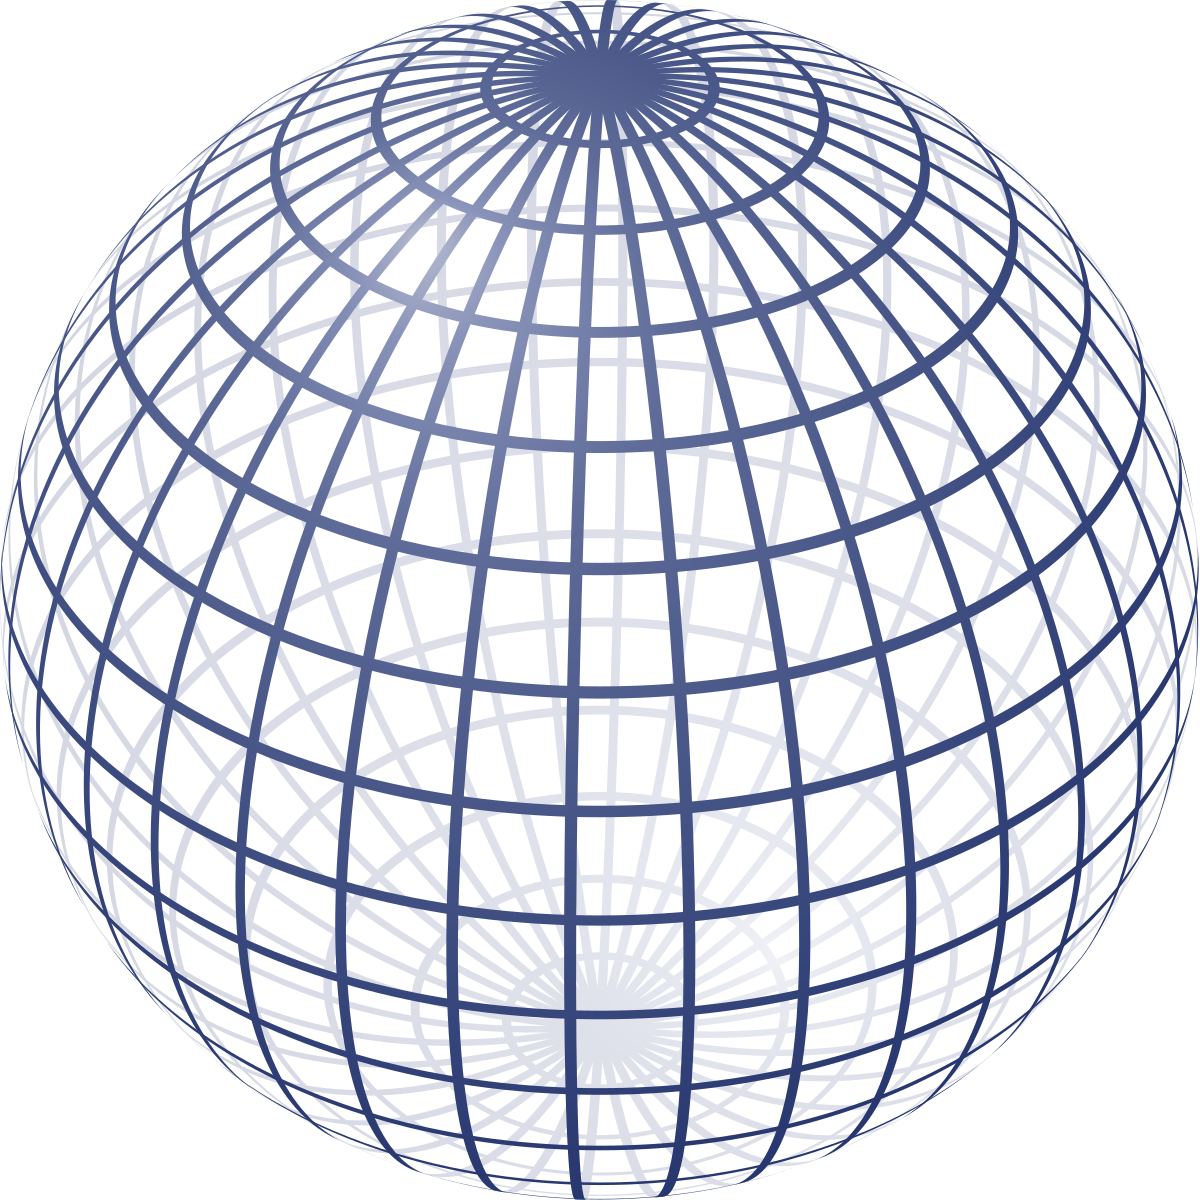
\includegraphics[scale=0.1]{sphere}
	\caption{Sfera. Źródło: \url{http://wikipedia.org}}
\end{figure}

Najważniejsze jest, aby umożliwić podróż wzdłuż równoleżników, natomiast symulacja podróży wzdłuż południków mogłaby być kłopotliwa do zrealizowania zakładając, że mapa jest ograniczoną płaszczyzną w kształcie kwadratu. Dlatego w ramach uproszczenia i częściowego zrealizowania działania mapy imitujący planetę mapa zostanie zapętlona wzdłuż granicznych "południków" tak, że logicznie przyjmie formę walca bez podstaw (czegoś na kształt rury).
\begin{figure}[h]
	\centering
	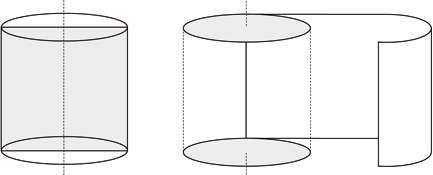
\includegraphics[scale=0.5]{walec}
	\caption{Sposób zwinięcia mapy w kształt walca. Źródło: \url{http://www.dachy.info.pl}}
\end{figure}

Oczywiście zwinięcie mapy w kształt walca w świecie gry realizowanym w 2D nie jest możliwe. Zostanie to zrealizowane poprzez niewidoczny dla gracza teleport z punktu $x\_max$ do punktu $-x\_max$ i na odwrót.
\subsection{Pogoda}
Zmienne pogodowe:
\begin{itemize}
	\item Temperatura będzie liniowo zmieniana w stosunku do pozycji $y$. Zakres temperatur to $+27^{\circ}C$ na równiku ($y = 0$) do $-133^{\circ}C$ na końcu biegunów ($|y| = y\_max$).\\
	Temperatura będzie obliczana z następującego wzoru:
	\begin{equation}
	\label{eqn:tempeq}
	temp = \ceil[\bigg]{-160\frac{|y|}{y\_max} + 27} [^{\circ}C]
	\end{equation}
	gdzie:\\
	\begin{tabular}{l l l}
	$y$ & - & odległość punktu od równika\\
	$y\_max$ & - & maksymalna możliwa odległość punktu od równika
	\end{tabular}
	\vspace{1em} \\ Niskie temperatury będą mogły wpływać na gracza oraz łaziki.
	\item Burze piaskowe będą przeszkadzać w łączności z łazikami. Wystąpienie burzy piaskowej będzie określone pewnym prawdopodobieństwem.
\end{itemize}
\subsection{Cykl dnia i nocy}
W cyklu dnia i nocy zostanie pominięty czynnik jakim jest przechylenie osi planety względem osi orbity wokół Słońca z racji uproszczenia mechaniki gry. Dzień i noc będą zajmowały po połowie długości doby. Długość doby zostanie określona na podstawie doświadczeń z wczesnych wersji gry.

Podczas nocy temperatura wynikająca ze wzoru \ref{eqn:tempeq} będzie dodatkowo pomniejszana o zadaną ilość stopni tak, aby utrudnić graczowi rozgrywkę nawet w niedalekiej odległości od równika.

Temperatura panująca w dzień będzie równa temperaturze wynikającej ze wzoru \ref{eqn:tempeq}.
\subsection{Badania}
\subsection{Cele gry}
\section{Programowanie łazików}
\end{document}
